\documentclass[a4paper,11pt]{article}

\usepackage[utf8]{inputenc} % allow utf-8 input
\usepackage{hyperref}       % hyperlinks
\usepackage{url}            % simple URL typesetting
\usepackage{booktabs}       % professional-quality tables
\usepackage{amsfonts}       % blackboard math symbols
\usepackage{nicefrac}       % compact symbols for 1/2, etc.
\usepackage{microtype}      % microtypography
\usepackage{graphicx}       % include graphics
\usepackage{subcaption}     % subfigures
\usepackage{float}          % placement of floats
\usepackage{fancyhdr}       % head notes and foot notes
\usepackage{bbm}            % Nice symbols
\usepackage{mathtools}      % Math tools like operators
\graphicspath{ {images/} }



\newcommand{\RR}{\mathbbm{R}} % Nice R sign
\DeclarePairedDelimiter\abs{\lvert}{\rvert} % abs
\DeclarePairedDelimiter\norm{\lVert}{\rVert} % norm
\DeclareMathOperator*{\argmin}{arg\,min} % argmin
\DeclareMathOperator*{\argmax}{arg\,max} % argmax

\title{Dictionary learning}


\author{
  Louis Martin\\
  \href{mailto:louis.martin@student.ecp.fr}{\tt louis.martin@student.ecp.fr}
}

\pagestyle{fancy}
\fancyhf{}
\lhead{Louis MARTIN}
\rhead{Sparsity and Compressed Sensing: Project}

\rfoot{Page \thepage}

\begin{document}

\maketitle

\begin{abstract}
%% Abstract (½ page):
%% What problem(s) is studied ?
This paper focuses on how to efficiently learn a dictionary in order to obtain a sparse representation of a signal (e.g. image or audio).
%% Why is it relevant ?
Deriving a sparse representation of a signal can be very efficient in solving multiple signal processing problems.
It has been successfully used in compression, inpainting, denoising, inverse problems and more.
One way to obtain a sparse coding is by using dictionaries.
A dictionary acts as a basis on which the data can be accurately represented using a small number of coefficients.
This basis can be either predefined or learned, both approaches have shown great results.
We will here focus how to efficiently learn an appropriate dictionary given the data we want to encode.
Finding a good dictionary is indeed important because it will define the representational power of the sparse coding,
i.e. how well the sparse coded signal will represent the original signal.
The learning process is therefore a key step for sparse representation.
%% What solution(s) is proposed ?
We propose to study and compare three different approaches to dictionary learning.
K-SVD algorithm which is proposed as a generalization of clustering algorithms such as k-means.
Online matrix factorization which provides an online approach to dictionary learning for big datasets.
An intuitive block coordinate projected gradient descent which is a specific case of the forward-backward proximal iterave method.
%% Which contributions (theory, numerics, etc) ?

\end{abstract}

\section{Introduction}
%% Introduction (~3 pages) :
%% Presentation of the problem(s).
Sparse coding is able to solve multiple signal processing tasks such as compression \cite{marcellin00}, inpainting, denoising \cite{elad06}, texture synthesis \cite{peyre09} and so on.
% Why do we want sparsity, i.e. a small number of non-zero coefficients ?
% 1) Compression
Sparsity, i.e. having a small number of non-zero coefficients, is wanted for several of its useful properties.

It is very effective for compression for obvious reasons of storage space, we only have to store a small set of sparse coefficients that will permit an accurate reconstruction if the original signal.
% 2) Theorem in the first lecture -> good compression coefficients => good denoising

Good compression coefficients also often implies good denoising properties.
Noise is indeed often small local high frequency and unstructured information that is pruned by the sparse coding.
% 3) Natural images tend to have a small number of non-zero coefficients.
% Complex images like random images (or lot of noise) or trees will have a higher number of coefficient.
Natural image tend to have a small number of non-zero coefficient whereas complex images like random images or images with trees will have a higher number of coefficients.
% Sparsity is the a good indicator of natural images
Sparsity is therefore a good indicator of natural images.

Given that having a sparse representation is useful, we want to pay particular attention to the choice of the space in which this representation lives.
The problem is often translated to finding a good basis for this space.
This basis of interest can either be predefined or learned.

One can use a predefined basis which will be fixed for all tasks and datasets such as the Fourier basis or the wavelet basis thanks to \cite{mallat99}.
The fact that such a basis does not depend on the data makes it hard to design but also powerful because it is universal can be reused and define a standard.
For example a good sparse representation of natural images in the wavelet space led to the success of the JPEG2000 algorithm for image compression, see \cite{marcellin00}.

Another approach is to learn the basis, which is what we will focus on in this paper.
From this point on we will interpret this basis as a dictionary for reasons that we will explain later.
A dictionary is a set of representative signals called atoms.
The signal of interest is therefore expressed as a linear combination of these atoms.

Having a learned dictionary that is specific to a certain type of data or to one image in particular can be very powerful.
The sparse representation can at the same time be sparser and represent the data better.
Another key idea is to design overcomplete dictionaries which means that there are more atoms than the each atom dimension and so these atoms are not linearly independent.
This is why the term basis to denote an overcomplete dictionary is abusive.
Designing overcomplete dicionaries gives more flexibility to the sparse representation and leads to easier problems than with an complete basis.
However with atoms that are non linearly independant, the decomposition is not unique as it would be with orthogonal basis such as Fourier or wavelet which makes the problem harder to solve analytically.
This is why we will study iterative approaches.

%% Previous works (at least a few citations). If relevant, include things that you have seen during the MVA course (or possibly other courses).
%% Contributions. Why is the studied method different/better/worse/etc. than existing previous works.

\section{Problem statement and previous work}
\subsection{Notations}
Given a signal of size $m$, \textbf{$y \in \RR^m$}, a dictionary is a collection of $k$ prototype signal atoms represented in a matrix $D \in \RR^{m \times p}$
We want to find $x \in \RR^p$, the sparse representation of $y$ in the dictionary $D$.
An representation $D x = y$ being often hard to find we will settle with an approximate representation $ D x \approx y$.
A sparse vector is a vector with a "small" number of non-zero coefficient, this is why the sparsity measure is the $l_0$ pseudo-norm denoted $\norm{.}_0$ which counts the number of non-zero coefficients.
The sparsity constraint then writes $\norm{x}_0<k$ with $k \in \mathbbm{N}$.

The problem we want to solve is therefore
$$\min\limits_{D \in \RR^{m \times p}, x \in \RR^p} \norm{y - Dx}_2^2  \text{  subject to  } \norm{x}_0<k$$


The sparsity measure, the $l_0$ pseudo-norm is non-convex which makes the problem hard to solve in many approaches like gradient descent because we are not guaranteed to find a minimum.
Given that $\forall p <1$, the $l_p$ pseudo-norm is non convex, the closest convex norm that we can use is the $l_1$ norm which is in practice a good measure of the sparsity of a signal compared to other norms.
This norm favors sparse representation as can be seen in figure \ref{l1l2_norm}.

\begin{figure}[!htbp]
\centering
  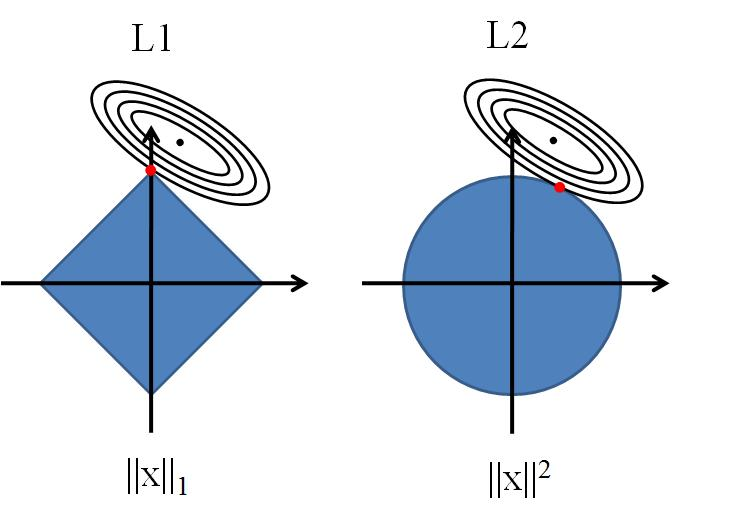
\includegraphics[width=0.5\linewidth]{l1l2_norm.jpg}
  \caption{The $l_1$ norm favors sparisty}
  \label{l1l2_norm}
\end{figure}

The constraint on $x$ will be represented by $x \in \chi_k = \{ x \in \RR^{p \times n}, \norm{x}_0<k \}$.
Furthermore we will want the dictionary to have normalized atoms.
Otherwise the atoms norm will increase for the sole purpose of decreasing the sparse representation norm and hence the $l_1$ constraint.
To prevent this behaviour from occuring we  will want $ D \in \mathcal{D} $ with $\mathcal{D} = \{ D \in \RR^{m \times p}, \forall i=1 \ldots p, \norm{D_{\cdot,i}} \leq 1 \}$.

We will often want to minimize the error over $n$ signals which will give us the problem :
$$\min\limits_{D \in \mathcal{D}, (x_i)_{i=1}^n \in \chi_k} \sum\limits_{i=1}^n \norm{y_i - Dx_i}_2^2$$
with $Y \in \RR^{m \times n}, Y = [y_1 \ldots y_n]$ and $X \in \RR^{p \times n}, X = [x_1 \ldots x_n]$.

The problem now rewrites in matrix form:
\begin{equation} \label{eq:1}
\min\limits_{D \in \mathcal{D}, X \in \chi_k} E(X,D) = \min\limits_{D \in \mathcal{D}, X \in \chi_k} \norm{Y - DX}_F^2
\end{equation}

Other methods like proximal methods will prefer rewriting \ref{eq:1} as:
$$\min_{X, D} E(X,D) + \iota_{\chi_k}(X) + \iota_{\mathcal{D}}(D)$$
with $\iota_C$ the indicator of set $C$ defined by
$ \iota_C(x) =
\begin{cases}
0, & \text{if } x \in C\\
+ \infty, & \text{otherwise}
\end{cases}
$

\subsection{Splitting the dictionary learning task into two subproblems}
Minimizing \ref{eq:1} both over $D$ and $X$ jointly is often not feasible.
That is why many approach split it into two subproblems that can be solved iteratively.
The first is to sparse code the data given the dictionary and the second to update the dictionary given this sparse coding. Fixing a variable and minimizing over the other was studied to work well in practice by \cite{lee06}.

\subsubsection{Finding the sparse representation}
This subproblem writes:
\begin{equation} \label{eq:2}
X \in \argmin_{X \in \chi_k} \norm{Y - DX}^2
\end{equation}
Equation \ref{eq:2} is typically solved by iterating over X until we have a solution that yields a small enough error $E(X,D)$.
Several alorithms called "pursuit algorithms" use this approach.

The most intuitive is matching pursuit which was introduced by \cite{mallat93} and successfully applied to signal decomposition.
The algorithm finds for each signal $y$, the atom $d_i$ which captures the most energy in the sense that
$$d_i = \argmax_{d_i \in D} |<y, d_i>|$$.
The corresponding coefficient is then set to $$x_i = \frac{<y, d_i>}{\norm{d_i}^2}$$ and the captured information is removed from $y$ so that $$y \leftarrow y - x_i d_i$$.
This process then is repeated until we reach the wanted sparsity or until the error is below a specified threshold.
A popular extension is orthogonal matching pursuit which updates all coefficients at each iteration. This leads to better results but also needs more computation.

Other pursuit algorithms are based on the matching pursuit approach and have shown great results such as FOCUSS for example.

Other successful approach using coordinate descent were successfully used as in \cite{wu08}, it is the type of approach that we used in the block coordinate gradient descent algorithm.

\subsubsection{Finding the dictionary}
PGD MOD
This part is the core of the dictionary learning problem and we will study it more in depth in the following sections.

The method of optimal directions from \cite{engan99} gives the optimal dictionary $D$ given a fixed $X$ with the update method:
$$ D^{i+1} = Y (X^{(i)})^T . (X^{(i)} (X^{(i)})^T)^{-1} $$
It however requires a matrix inversion which is impractical for large dictionaries.


\section{Dictionary learning methods}
%% Main body (~10 pages) :
%% Presentation of the method(s).
%% Theoretical guarantees.
%% Numerics.
Most of the iterative methods are composed of the two steps defined above.
Sparse coding the vector and updating the dictionary given this sparse representation.


\subsection{Proximal methods}
A intuitive and efficient algorithm for dictionary learning is to use a block coordinate gradient descent approach as in implemented in \cite{nt4} and is shown to converge in \cite{tseng01}.
This algorithm is part of the category of proximal methods and has gained substantial attention in signal processing \cite{combettes11}.
This is a two step algorithm.
We initialize $n$ training signals $(y_i \in \RR^m)_{i=1}^{n}$
that we put in a matrix $Y \in \RR^{m \times n}, Y = [y_1 \ldots y_n]$.
\begin{itemize}
  \item First we find the best sparse representation of the data given a fixed dictionary.
  	\begin{equation} \label{eq:pgd1}
      X^{(i+1)} \in \argmin_{X \in \chi_k} \norm{Y - D^{(i)}X}^2
	\end{equation}
  \item Then we update the dictionary given this sparse representation.
  	\begin{equation} \label{eq:pgd2}
      D^{(i+1)} \in \argmin_{D \in \mathcal{D}} \norm{Y - DX^{(i+1)}}^2
	\end{equation}
\end{itemize}


\subsubsection*{Forward-Backward algorithm}
\ref{eq:pgd1} and \ref{eq:pgd2} can be solved using the Forward-Backward proximal algorithm which is detailed in \cite{combettes11}, \cite{parikh14} and in the class lectures.
We have
\begin{equation*}
\begin{split}
x^* \in \argmin_x F(x) + G(x) & \Longleftrightarrow 0 \in \nabla F(x^*) + \partial G(x^*)\\
							  & \Longleftrightarrow (x^* - \gamma \nabla F(x^*)) \in x^* + \gamma \partial G(x^*)\\
                              & \Longleftrightarrow x^* = Prox_{\gamma G} (x^* - \gamma \nabla F(x^*))
\end{split}
\end{equation*}

The Forward-Backward update thus reads
$$x^{(i+1)} = Prox_{\gamma G} (x^{(i)} - \gamma \nabla F(x^{(i)})$$
with the proximal operator being an natural extension of the projection on a convex set.
$$Prox_{\gamma G}(x) = \argmin_z \frac{1}{2} \norm{x - z}^2 + \gamma G(z)$$

When $G = \iota_C$ then the proximal operator is the projection on the convex set C.
$$Prox_{\gamma G}(x) = \argmin_{z \in C} \norm{x - z} = \Pi_C(x)$$
In this special case, Forward-Back is equivalent to \emph{projected gradient descent}

\ref{eq:pgd1} and \ref{eq:pgd2} can be rewritten as
$$\argmin_X E(X,D) + \iota_{\chi_k}$$
$$\argmin_D E(X,D) + \iota_{\mathcal{D}}$$

We thus only need compute the gradient of $E(X,D)$ with respect to X and D and apply the Forward-Backward update rule to finally have:

$$ X^{(i+1)} = X^{(i)} - \gamma D^T (D^{(i)}X^{(i)} - Y) $$
$$ D^{(i+1)} = D^{(i)} - \tau (D^{(i)}X^{(i+1)} - Y) X^T $$

\begin{figure}[!htbp]
\centering
  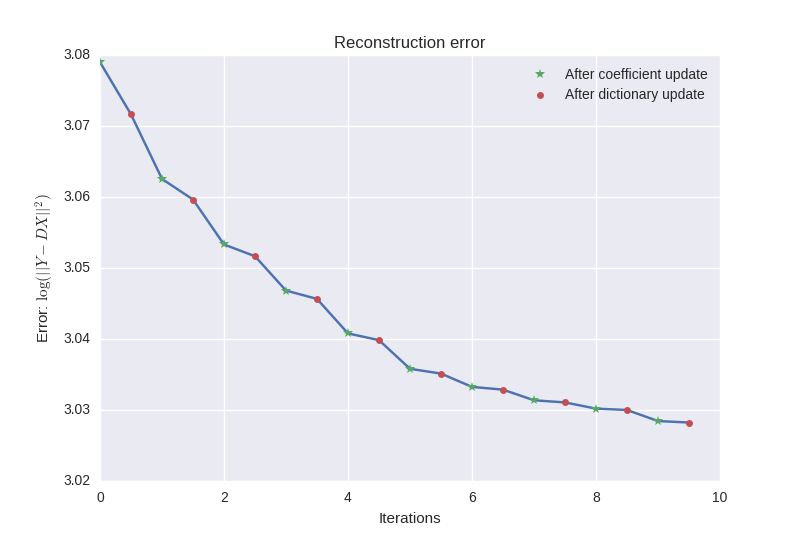
\includegraphics[width=\linewidth]{fb_12_iter_synthetic.png}
  \caption{Implementation of Forward-Backward on synthetic data.}
\end{figure}

\subsection{K-SVD}
The approach in \cite{aharon06} is interesting in the way that it considers the dictionary learning problem as a generalization of a clustering problem. Clustering is indeed an extreme case of sparse coding where there is only one non-zero coefficient and this coefficient must be one.

The K-SVD algorithm can be used with any sparse coding technique because it is focused on the dictionary update.
Each column $d_k$ of the dictionary is updated independently takes to a good decomposition of the error $E(X,D)$ into a matrix that does not depend on $d_k$ and a rank 1 matrix that does.
\begin{equation} \label{eq:ksvd1}
\begin{split}
  E(X,D) & = \norm{Y - DX}_F^2 \\
  		 & = \norm{Y - \sum\limits_{j=1}^{p} d_j x^j} \text{ ($x^j$ is the $j$th row, not the column $x_j$)}\\
         & = \norm{(Y - \sum\limits_{j \neq k} d_j x^j)  - d_k x^k}
\end{split}
\end{equation}

We will then subset these matrices to only keep the parts that use the column $d_k$.
That is why the ensemble $\omega_k = \{i | i = 1 \ldots N, x^k(i) \neq 0\}$, is introduced. It denotes the indices of the samples that use the atom $d_k$.
Using this ensemble we can construct the matrix $\Omega_k \in N \times |\omega_k|$ with ones at the $(\omega_k(i),i)$ coordinates and zeros everywhere else.

This matrix will subset the problem to only the values concerned by the update of the column $d_k$.

We can now rewrite the minimization of the error defined in \ref{eq:ksvd1} as
\begin{equation*}
\begin{split}
  \min_{d_k \in \mathcal{D}, x^k \in \chi_k} \norm{E_k - d_k x^k }_F^2 & = \min_{d_k \in \mathcal{D}, x^k \in \chi_k} \norm{E_k \Omega_k - d_k x^k \Omega_k}_F^2 \\
  											& = \min_{d_k \in \mathcal{D}, x^k_R} \norm{E_k^R - d_k x^k_R}_F^2 \\
                                            & \text{ (with $E_k^R$ and $x^k_R$ only values concerned by $d_k$)}
\end{split}
\end{equation*}

Note that we optimize on both $d_k$ and $x^k_R$ at the same time. The restriction of $x^k$ to $x^k_R$ also forces it to have the same support before and after the update so that we don't need to explicitely enforce the sparsity constraint.
This basically boils down to finding the best rank one matrix approximation of $E_k^R$.
With $E_k^R = U \Delta V^T$ being the SVD decomposition of $E_k^R$, Eckart–Young–Mirsky theorem states that $\sigma_1 u_1 v_1^T$ is the best rank one approximation of $E_k^R$.\\
The update rule is therefore $d_k \leftarrow u_1$ and $x^k_R \leftarrow \sigma_1 v_1$.
This step is repeated for all the columns as it is done for the means in K-means thus the name K-SVD.

\begin{figure}[!htbp]
\centering
  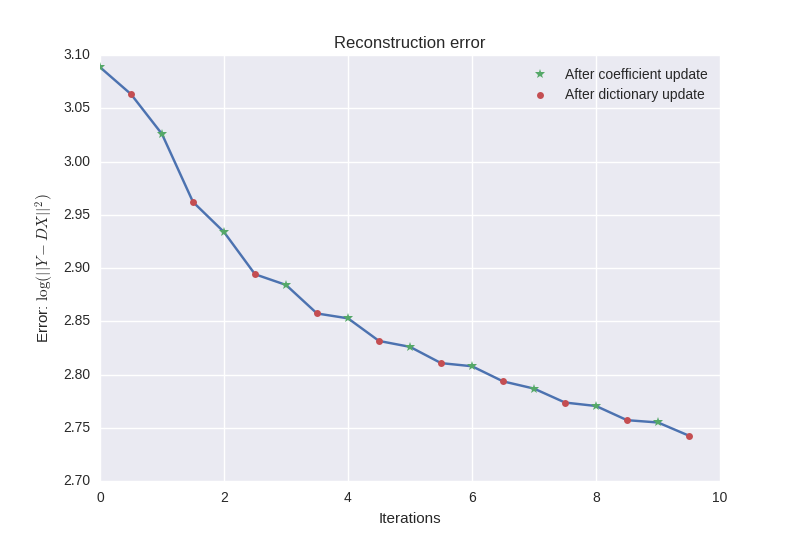
\includegraphics[width=\linewidth]{ksvd_12_iter_synthetic.png}
  \caption{Implementation of K-SVD on synthetic data.}
\end{figure}



\subsection{Online learning for matrix factorization}
\ref{eq:1} can be interpreted as a matrix factorization problem. Indeed we try to find a factorization of $Y$ in the form $DX$.
When confronted with a very large number of samples $N$, it is impractical to work directly with the $Y$ and $X$ matrices. That is why \cite{mairal10} proposes to solve the problem iteratively, sample by sample in an online fashion. Online learning also reduces overfitting if given a big enough dataset.

The method proposed draws random samples as in stochastic gradient descent, derive its sparse representation and then updates the dictionary.
However the objective is to not only update the dictionary based on the current sample but also on all the samples that we previously considered in order to have a more substantial update.
The sparse coding step is done using the $l_1$ penalty with LARS-lasso algorithm from \cite{efron04}.

Let's rewrite the update rule in a form that will lead to an efficient algorithm.
\begin{equation*}
\begin{split}
  D_t & = \argmin_{D \in \mathcal{D}} \frac{1}{t} \sum\limits_{i=1}^t (\frac{1}{2} \norm{y_i - D x_i}_2^2 + \lambda \norm{x_i}_1)\\
      & = \argmin_{D \in \mathcal{D}} \frac{1}{t}  (\frac{1}{2} \norm{Y_t - DX_t}_F^2 + \lambda \norm{X_t}_{1,1})\\
      & = \argmin_{D \in \mathcal{D}} \frac{1}{t}  (\frac{1}{2} \norm{Y_t - DX_t}_F^2) \text{   ($\norm{X_t}_{1,1}$ does not depend on $D$)}\\
      & = \argmin_{D \in \mathcal{D}} \frac{1}{t}  (\frac{1}{2} Tr((Y_t - DX_t)^T (Y_t - DX_t)))\\
      & = \argmin_{D \in \mathcal{D}} \frac{1}{t}  (\frac{1}{2} Tr(Y_t Y_t^T) - Tr(X_t^T D^T Y_t) + \frac{1}{2} Tr(X_t^T D^T D X_t))\\
      & = \argmin_{D \in \mathcal{D}} \frac{1}{t}  (\frac{1}{2} Tr(D^T D X_t X_t^T) - Tr(D^T Y_t X_t^T) )\\
      & = \argmin_{D \in \mathcal{D}} \frac{1}{t}  (\frac{1}{2} Tr(D^T D A_t) - Tr(D^T B_t) )
\end{split}
\end{equation*}

We can decompose $A_t$ and $B_t$ as follows:
$$ A_t = \sum\limits_{i=1}^t x_i x_i^T \text{ and } B_t = \sum\limits_{i=1}^t y_i x_i^T $$
We can therefore update $A_t$ and $B_t$ for each sample and not compute them from scratch every time.

We can then update each column independently with:
$$ u_j \leftarrow \frac{1}{A[j,j](b_j - D a_j) + d_j} $$
$$ d_j \leftarrow \frac{1}{\max(\norm{u_j}_2, 1)} u_j $$

This algorithm is shown to converge to a solution $D^*$ and note that it does not depend on any paramater such as a learning rate.

\section{Results}
\subsubsection*{Synthetic data}
We tested the algorithms on synthetic data.
We generate signals $Y$ from a given dictionary $D$ and sparse coefficients $X$. The algorithms are then given only $Y$ and have to find an appropriate sparse representation of $Y$ by learning a dictionary.
The parameters used for this synthetic data are:
$$signal\_size=25, n\_atoms=50, n\_samples=1000, sparsity=4$$

\subsubsection*{Sparse coding}

\begin{figure}[!htbp]
\begin{tabular}{|c|c|c|c|}
  \hline
  & OMP & Lasso & FB \\ \hline
  Speed & 940 ms & 270 ms & 870 ms \\ \hline
  $E(X,D)$ & 7 & 230 & 284 \\ \hline
\end{tabular}
  \caption{Evaluation of Orthogonal matching pursuit, Lasso, and Forward-backward (100 iterations) on synthetic data. We evaluate the speed for one step and the reconstruction error of the sparse coding after this step.}
  \label{sparse_coding_perfs}
\end{figure}
We evaluated the speed and reconstruction error after one sparse coding step for Orthogonal matching pursuit, lasso regression, and the forward-backward scheme in figure \ref{sparse_coding_perfs}.
The result are not to be taken as ground truth because the number of samples is very small and there are several parameters that could have been tweaked for the different algorithms. An extensive benchmark should be run.
However we can see that orthogonal matching pursuit is better at finding a sparse representation and lasso is pretty fast in these settings. Orthogonal matching pursuit seems a reliable choice for sparse coding the data.

\subsubsection*{Dictionary learning}

\begin{figure}[!htbp]
\centering
  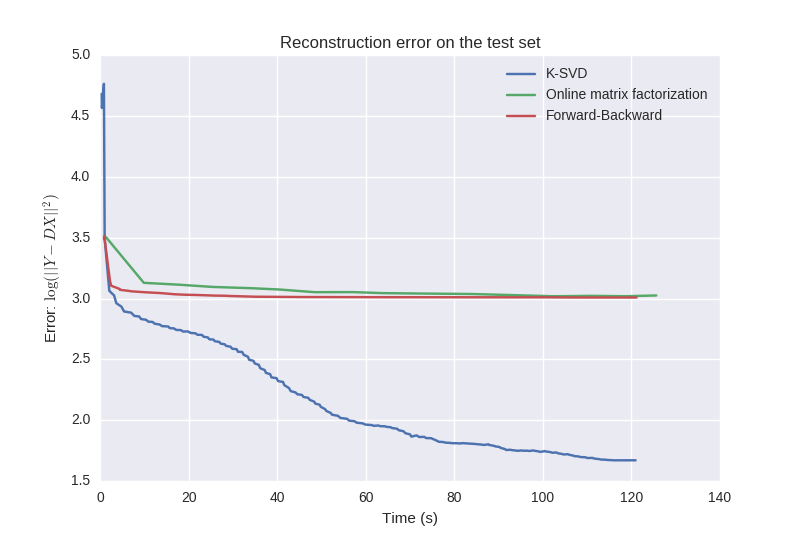
\includegraphics[width=\linewidth]{comparison_120s_synthetic.png}
  \caption{Comparison of the three algorithms}
  \label{comparison}
\end{figure}

We ran the three algorithm on synthetic data, namely (sparse coding - dictionary update):
\begin{itemize}
  \item Orthogonal matching pursuit - K-SVD
  \item Lasso - Online matrix factorization
  \item Forward-Backward (for both)
\end{itemize}
The algorithms were timed and the reconstruction error tracked which gave the results displayed on figure \ref{comparison}.
It seems that both Online matrix factorization and Forward-Backward seem to plateau and decrease ever so slowly from a point whereas K-SVD gives very good results and continue learning while the others are stuck.
However the pros of online matrix factorization is that it can handle large amount of samples whereas the others cannot.
This might be why it does not perform as well on small datasets, solving the problem sample by sample is indeed slower.
Forward-Backward algorithm is the only algorithm with a learning rate that would probably give better results if dynamically adapted to the evolution of the error.

What we can take out of this experiment is that K-SVD might be the best suited algorithm for small dataset like patches of an image, it outperforms the two other algorithms probably because of its clever update
On the other hand, online matrix factorization is way more adapted for large datasets and online learning.

\section{Conclusion}
%% Conclusion and perspective (~1 page)
%% Summary of the result obtained: pros and cons (limitation, problems, error in the articles, etc)
%% Possible improvement/extension
Dictionary learning can be used in a wide array of signal processing tasks, that is why it is important to find efficient and accurate methods to learn appropriate dictionaries.
The algorithm studied each have their particularities. K-SVD seems to be the best bet because it is both fast and accurate. Forward-Backward's update rule is more intuitive but might need more learning rate tinkering. Finally, online matrix factorization is more adapted to online learning and very large datasets. It can even be improved by several modifications proposed in \cite{mairal10} like mini-batch training.

\subsubsection*{Application to real image}

\begin{figure}[!htbp]
\centering
  \begin{subfigure}[b]{.35\linewidth}
    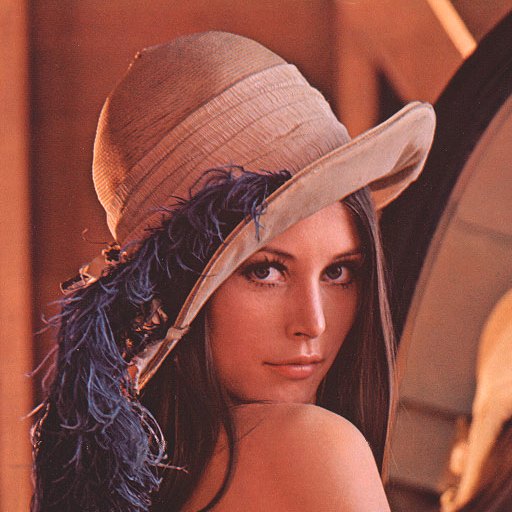
\includegraphics[width=\linewidth]{lena.png}
    \caption{Natural image used to sample patches to learn a dictionary.}
  \end{subfigure}
  \begin{subfigure}[b]{.6\linewidth}
    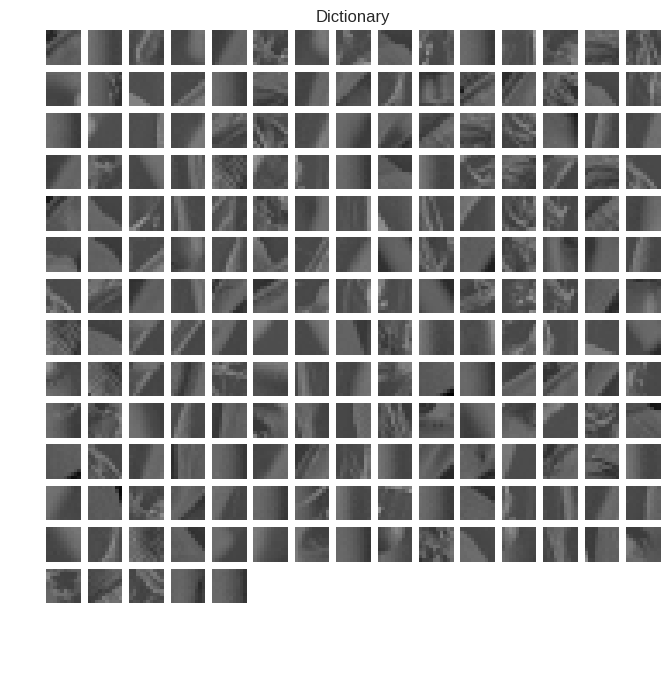
\includegraphics[width=\linewidth]{dict_lena.png}
    \caption{Centered dictionary learnt by K-SVD}
  \end{subfigure}
  \label{dict_lena}
\end{figure}

We applied the K-SVD algorithm on 10x10 patches of a natural image.
The resulting dictionary in figure \ref{dict_lena} shows interesting patterns.
It seems that the algorithm prefered atoms with higher energy with oriented edges.
Their representation power is indeed higher than smoother patches, it is easier to represent shapes with edges.

\begin{thebibliography}{9}
%% Bibliography (~1 page)

\bibitem{elad06}
Elad, Michael, and Michal Aharon. "Image denoising via sparse and redundant representations over learned dictionaries." IEEE Transactions on Image processing 15.12 (2006): 3736-3745.

\bibitem{peyre09}
Peyré, Gabriel. "Sparse modeling of textures." Journal of Mathematical Imaging and Vision 34.1 (2009): 17-31.

\bibitem{lee06}
Lee, Honglak, et al. "Efficient sparse coding algorithms." Advances in neural information processing systems. 2006.

\bibitem{gorodnitsky97}
Gorodnitsky, Irina F., and Bhaskar D. Rao. "Sparse signal reconstruction from limited data using FOCUSS: A re-weighted minimum norm algorithm." IEEE Transactions on signal processing 45.3 (1997): 600-616.

\bibitem{mairal10}
Mairal, Julien, et al. "Online learning for matrix factorization and sparse coding." Journal of Machine Learning Research 11.Jan (2010): 19-60.

\bibitem{aharon06}
Aharon, Michal, Michael Elad, and Alfred Bruckstein. "K-SVD: An Algorithm for Designing Overcomplete Dictionaries for Sparse Representation." IEEE Transactions on signal processing 54.11 (2006): 4311-4322.

\bibitem{mallat99}
Mallat, Stéphane. A wavelet tour of signal processing. Academic press, 1999.

\bibitem{mallat93}
Mallat, Stéphane G., and Zhifeng Zhang. "Matching pursuits with time-frequency dictionaries." IEEE Transactions on signal processing 41.12 (1993): 3397-3415.

\bibitem{marcellin00}
Marcellin, Michael W., et al. "An overview of JPEG-2000." Data Compression Conference, 2000. Proceedings. DCC 2000. IEEE, 2000.

\bibitem{olshausen97}
Olshausen, Bruno A., and David J. Field. "Sparse coding with an overcomplete basis set: A strategy employed by V1?." Vision research 37.23 (1997): 3311-3325.

\bibitem{tseng01}
Tseng, Paul. "Convergence of a block coordinate descent method for nondifferentiable minimization." Journal of optimization theory and applications 109.3 (2001): 475-494.

\bibitem{parikh14}
Parikh, Neal, and Stephen P. Boyd. "Proximal Algorithms." Foundations and Trends in optimization 1.3 (2014): 127-239.

\bibitem{efron04}
Efron, Bradley, et al. "Least angle regression." The Annals of statistics 32.2 (2004): 407-499.

\bibitem{combettes11}
Combettes, Patrick L., and Jean-Christophe Pesquet. "Proximal splitting methods in signal processing." Fixed-point algorithms for inverse problems in science and engineering. Springer New York, 2011. 185-212.

\bibitem{wu08}
Wu, Tong Tong, and Kenneth Lange. "Coordinate descent algorithms for lasso penalized regression." The Annals of Applied Statistics (2008): 224-244.

\bibitem{engan99}
Engan, Kjersti, Sven Ole Aase, and J. Hakon Husoy. "Method of optimal directions for frame design." Acoustics, Speech, and Signal Processing, 1999. Proceedings., 1999 IEEE International Conference on. Vol. 5. IEEE, 1999.

\bibitem{nt4}
Peyré, Gabriel. "Numerical tours - Dictionary learning",
\href{https://github.com/gpeyre/numerical-tours/blob/master/matlab/sparsity_4_dictionary_learning.ipynb}{url}

\end{thebibliography}
\end{document}

% Information for the project report:
% If possible, write the report in english.
% You must bring a printed version with your to give me before the presentation. This is a strict deadline.
% Using Latex is highly recommended.
% Roughly 15 pages (A4, 11pt font, single column), including roughly one page of bibliography.
% Should be similar to a (short) scientific article in an applied mathematics journal.
% No source code.
% When presenting the numerics, give all parameters, so that the results are reproducible.
% It should not be a rewriting of the original article. You should only report about what you have done, and only explain the theory that is relevant to explain the numerics you have done.
% Suggestion of structure for the report:
% Abstract (½ page):
% What problem(s) is studied ?
% Why is it relevant ?
% What solution(s) is proposed ?
% Which contributions (theory, numerics, etc) ?
% Introduction (~3 pages) :
% Presentation of the problem(s).
% Previous works (at least a few citations). If relevant, include things that you have seen during the MVA course (or possibly other courses).
% Contributions. Why is the studied method different/better/worse/etc. than existing previous works.
% Main body (~10 pages) :
% Presentation of the method(s).
% Theoretical guarantees.
% Numerics.
% Conclusion and perspective (~1 page)
% Summary of the result obtained: pros and cons (limitation, problems, error in the articles, etc)
% Possible improvement/extension
% Bibliography (~1 page)
